\section{Implementation}

My implementation is in two parts: that of the protocol described above, and additionally an example \textit{Web3} client. The protocol itself is split between peer-to-peer communication and smart contract methods. P2P messages are handled entirely outside of the contract, and in this implementation are sent by the client library via the Whisper protocol on the Ethereum network.

The entire implementation of the Taxicoin protocol and client is contained within one git repository. The directory structure is defined by a combination of \lstinline{vue-webpack} \cite{VueWebpack} and \lstinline{truffle} \cite{Truffle}, both of which have strong opinions.

\subsection{Smart Contract}

As previously discussed, Ethereum smart contracts are self-contained programs which execute on the Ethereum Virtual Machine (EVM). The core of Taxicoin is implemented as a contract, allowing riders and drivers to interact with one and other with it as an intermediary.

The contract is centred around state, which can be divided into three parts: the state of the Taxicoin network, the state of a driver, and the state of a rider. It conforms to the \lstinline{TaxicoinInterface} contract interface, as defined in the protocol specification.

\subsubsection{Network State}

When a contract is deployed, various parts of it may be initialised, in a similar way to how the constructor of a class initialises the state of an object. In Taxicoin, only the driver and rider deposit values are set at this stage.

Two key mappings are kept: one which maps an address to a driver, and one which maps an address to a rider. There is additionally a third mapping used to implement a double-linked list (DLL), discussed below.

There is also a \lstinline{UserType} enum from the contract interface, which is used as a return type for the \lstinline{getUserType} helper function. This is an easy method of determining the current \enquote{mode} of a user based on the state of their \lstinline{Driver} and \lstinline{Rider} objects (described in more detail below).

\lstinputlisting[language=Solidity]{res/user-type-enum.sol}

\subsubsection{Driver State}

An individual driver is represented by a \lstinline{Driver} struct:

\lstinputlisting[language=Solidity]{res/driver-struct.sol}

When a user first wishes to become a driver, a \lstinline{Driver} object will not exist for them\footnotemark, and they will have to call the \lstinline{driverAdvertise} method, providing their current latitude, longitude, Whisper public key (used for peer-to-peer communication), and a deposit. If the deposit provided is sufficient, then the driver's state will be updated.

\footnotetext{Rather, the mapping will return a Driver object with all zero values.}

This consists of setting the address of the driver on the object (used as an integrity check - the address of an advertised driver should map to a \lstinline{Driver} object with the same address), the latitude and longitude, the time at which the driver was last updated (used to detect stale advertisements), the deposit provided by the driver (for cases where the global driver deposit value may change, the amount provided when the driver initially advertised is what will be returned), and the driver's public key (used for contacting this driver via Whisper). Additionally, if the driver is not already advertised, their address is added to the DLL.

Just as the address of a \lstinline{Driver} object is used to check integrity, it is also used to indicate whether a driver is currently advertised or not. Any user should be able to view information about a driver at any time, and the overall rating of a driver needs to be stored even while a driver is not advertised. Therefore, this data is kept, and can be accessed via the \lstinline{drivers} map. However, if the address does not match, this indicates that the driver is not currently advertised.

To mark a driver as not active, they are removed from the DLL and their address set to zero. To mark a driver as on a journey, they are removed from the DLL and their rider is set to a non-zero address. The advantage of this state-based approach to determining the mode of a driver is that we do not have to explicitly store and update a separate indicator.

\subsubsection{Rider State}

An individual rider is represented by a \lstinline{Rider} struct:

\lstinputlisting[language=Solidity]{res/rider-struct.sol}

A rider's rating and rating count are kept between journeys, but otherwise, all remaining fields are empty when the rider is not part of a journey. As with a driver, the \lstinline{addr} field is used to determine whether a rider is active. To determine whether the driver is locked into a journey, we look up the driver in the \lstinline{drivers} mapping, using the given address. If their rider field is set to the address of this rider, then both users are locked into a rider together.

\subsubsection{Double Linked List}

As Solidity is still a relatively young language, some features which one would expect from a more mature language are missing. This includes the ability to return dynamic-length lists from a method, which posed an issue early in the development of Taxicoin. Although it's possible to return a single element at a time, this requires keeping a separate cursor for which element should be next. Therefore we instead use a novel implementation of a double-linked-list, which allows us to use the address of the current driver as the cursor to fetch the next or previous\footnotemark.

\footnotetext{The ultimate implementation was based on \cite{DLL}.}

Modifying operations on the list are likely be performed on only a single element at a time, therefore to link to the next and previous item in the list is not much more of a cost. This provides the benefit of not having to scan forward to move backwards in the list, particularly useful for pagination, which will likely be needed when a large number of drivers are advertised and a user wishes to manually review potential drivers.

The contract uses a mapping which maps driver addresses to another map, which in turn maps a boolean to an address. The boolean represents whether we want to look up the next or previous element in the list - false is the previous, and true is the next. This then returns the address to use to look up the \lstinline{Driver} object in the drivers mapping.

This list is easily interfaced with using the \lstinline{getNextDriver} and \lstinline{getPreviousDriver} methods, as defined in the contract interface. These features of the protocol were in fact partly designed this way due to the limitation as described above, that solidity does not support returning dynamic-length lists from methods.

\subsubsection{Journeys}

Building on the idea of rider and driver state, there is no concrete \textit{journey} object in this Taxicoin implementation. Rather, the concept of a journey is inferred from the state of the participants.

When observing a rider, if the \lstinline{driver} property is set, this indicates that the driver is either on a journey with that driver, or has created the journey and is waiting for the driver to accept. Whether the driver has accepted or not can be determined by observing the driver's \lstinline{rider} property. If it is set the address of the rider, then the driver has accepted the journey and both are formally part of the same journey. If the driver's rider address is blank, they have not yet accepted the journey, and if it is the address of another rider, then they have effectively declined the journey with this rider and have chosen to accept another rider's journey.

At the end of a journey, both parties call the \lstinline{Complete Journey} method, which will record the rating to be given to the other. This is stored in the rider/driver object for the user, and additionally acts as an indication as to whether the user has already called the method. This is then used by the method to determine whether to finalise the completion of the journey.

When both parties have completed the journey, the ratings given are applied (recalculate average rating, and increment rating count), deposits returned, and the fare paid to the driver. The state of both is then reset -- their own addresses and those pointing to the other are set to zero, the ratings to be given to the other are set to zero, and the recorded values for the deposits are fare are set to zero.

\subsubsection{Integrity Checks}

As this implementation is heavily based on the state of objects within the contract, it is important to maintain data integrity. Coupled with the immutability of smart contracts, if we do not ensure that our contract state is kept correctly, it may be impossible to recover from a situation where the state is altered in some unexpected way.

A key feature of Solidity which allows us to check certain pre- and post-conditions is the use of \lstinline{require();}. In the case that the contained statement evaluates to false, execution will halt and any changes made to the state of the contract instance are reverted.

For example, the protocol specification states that when a driver advertises, they must first be required to pay a deposit. Additionally, they may not already be on a journey as either a driver or rider. To check these post-conditions we can use the following Solidity code:

\begin{lstlisting}[language=Solidity]
// check the driver has paid deposit
require(drivers[msg.sender].deposit >= driverDeposit || msg.value >= driverDeposit);

// must not be ActiveDriver or Rider
require(getUserType(msg.sender) != UserType.ActiveDriver);
require(getUserType(msg.sender) != UserType.Rider);
\end{lstlisting}

This is also useful for performing \enquote{safe math}, where we want to protect against overflow or underflow. In both of these cases, integers in Solidity will simply wrap-around, which, particularly when dealing with currency as is the case much of the time in Solidity, can be catastrophically bad. Although it may not always be possible to recover from a situation where over- or underflow would occur, we can use \lstinline{require} to check if the resulting value has been a result of such an occurrence, and revert the state of the contract instance.

\subsection{Client Library}

While the contract handles the state of Taxicoin, it can be unwieldy to interact with. It also only implements part of the Taxicoin protocol, not including any of the off-chain, peer-to-peer interactions.

The JavaScript client library is what really opens up the potential ecosystem of applications using the Taxicoin protocol. The aim was for it to be as simple to use and integrate into other people's projects as possible, and ideally should hide as much of the complexity of interacting with an Ethereum smart contract as possible.

The client library exposes a class, which when instantiated sets up all of the common requirements for using the Taxicoin protocol in most cases.

\subsubsection{Web3 Interaction}

The JavaScript library used for interacting with the Ethereum blockchain is called \lstinline{Web3.js} \cite{Web3}, and acts as a layer for sending commands to an Ethereum network node which computes transactions and relays them to the network.

This is coupled with the \lstinline{truffle-contract} library, which abstracts the logic for calling methods of a smart contract, and provides each one as an asynchronous JavaScript method. These in turn interact with a Web3 library instance. The typical code\footnotemark for calling a contract method is as follows:

\footnotetext{In ES6 async/await function syntax.}

\begin{lstlisting}
const instance = await this.contract.deployed()
const account = await this.getAccount()
const tx = await instance.methodToCall([arguments, ]{from: account[, otherOptions})
\end{lstlisting}

\lstinline{this.contract} is a \lstinline{TruffleContract} instance which points to the Taxicoin contract code. Calling the \lstinline{deployed} method on that returns a wrapper with a reference to a deployed instance of the contract on the current network. From this, we can then call the methods of the deployed contract.

The \lstinline{getAccount} method fetches the Ethereum address of the user, as defined when instantiating a Taxicoin library instance. This is then required to be passed as an option with any contract method calls which modify state, as it is used to identify the user when signing the transaction.

\subsubsection{Peer to Peer Messages}

The other key purpose of the client library is to facilitate the sending of peer-to-peer Taxicoin protocol messages. This is done with Whisper, one of the protocols part of the Ethereum network.

As Whisper is a fairly low-level protocol, sending messages is not entirely straightforward. The Web3 library handles much of the work, however it still requires various parameters, such as keys and the level of encryption it should use. Topics in Whisper also must be exactly 4 bytes in length, and the Web3 library expects this as a hexadecimal string, which is not something that would be straightforward for a user of the Taxicoin library.

Therefore, the library manages the keypair for use with Whisper, maps human-readable topic names to 4 byte hexadecimal string, converts JSON objects to strings for sending as the payload of a message, and handles the various other parameters used when sending Whisper messages.

For messages which are intended to be send after certain on-chain actions are taken, the library handles this, waiting for the transaction to be confirmed, and sending the appropriate message.

The library also registers filters for the various Taxicoin message topics, automatically polls for new messages sent to the user, and fires JavaScript events which the user of the library may listen for in their application.

\subsection{Example Web Client}

The example client implementation uses the client library, along with \textit{Web3.js} to interact with the Ethereum blockchain and Whisper protocol.

The \textit{Vue.js} JavaScript framework is used as a basis on which to develop a single-page web application. Vue uses a component-based architecture, where the functionality and formatting for a component is all self-contained. Pages are also considered to be components, and therefore each page follows the same model.

The application is split into two main parts: the ride page, and the drive page. Each one features user interface elements specific to that type of user.

\begin{figure}[h]
	\centering
	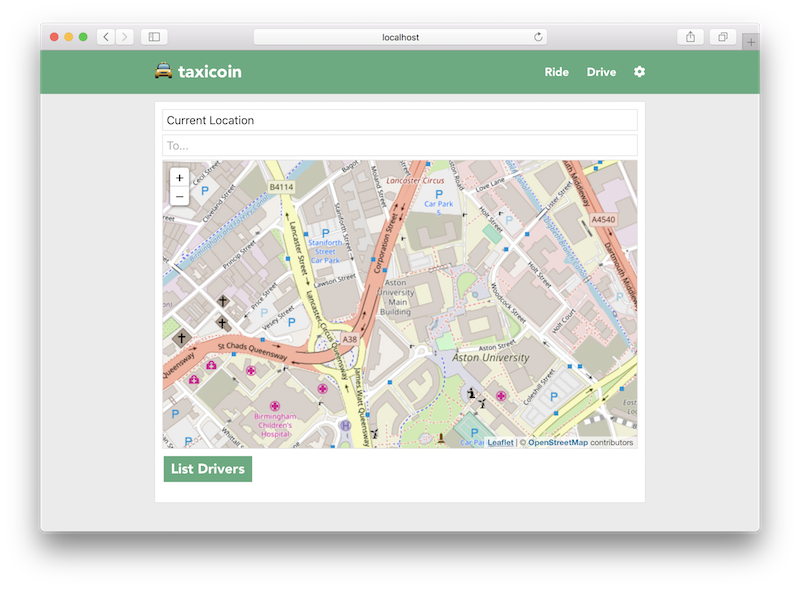
\includegraphics[width=11cm]{res/webapp.png}
	\caption{The example Taxicoin client, as viewed in the Safari browser.}
\end{figure}

Vue introduces the concept of \textit{reactive} data - when a JavaScript object changes value, any component which is using the data (observing it) automatically updates to use the new value. Retrieving the user's current location is a key requirement for any implementation of the Taxicoin protocol, and within a web browser this can be done using the geolocation browser API.

To adapt this for use with Vue's reactive models, a Vue \textit{plugin} has been created as part of this implementation. This creates a \lstinline{$location} object available to all components globally, which has latitude and longitude components, both of which are reactive.

Another plugin was also created for exposing a Taxicoin library instance to all components. This means that instead of needing to instantiate this for each page components and then pass it to child components where needed, the one instance is available globally.

Although this client implementation is functional, it is not feature complete at the time of writing, and does not implement all features of the library, such as sending of the driver's location to the rider, or a user interface for proposing a fare alteration. However, it is sufficient as a proof of concept.

Additionally, this application is most likely to be used from a mobile device (very few taxi drivers carry a laptop with them). This is possible using the Status mobile Ethereum browser \cite{Status.im}, which exposes a Web3.js object to web pages (also including Whisper protocol functionality, and in fact pioneering the 6th iteration of the protocol).
